\chapter{등각 사상과 열린 끈 산란 처방}

\lectureoverview{등각 사상은 처음에는 2차원 정전기학에서 유용한 대칭으로 등장한다. 복소 미분 가능성은 이 대칭을 계산 가능한 것으로 만든다. 코시--리만 방정식은 라플라스 방정식을 함의하고, 방향에 무관한 복소 미분 계수는 각도를 보존한다. 이 도구를 갖추면 끈 세계면을 띠, 반평면, 원통 또는 원판으로 그려도 물리는 바뀌지 않는다. 이어서 열린 끈 산란은 원판 경계에 운동량 삽입을 둔 가우스 경로 적분을 계산하고, 서로 동등하지 않은 삽입 위치에 대해 적분하는 문제로 바뀐다.}

\section{2차원 세계의 정전기학}

먼저 문자 그대로의 2차원 정전기 문제를 생각하자. 전하와 전기력선은 평면에 갇혀 있으며, 단지 운동이 평면에 한정된 보통의 3차원 전하를 뜻하는 것은 아니다. 그러면 가우스 법칙으로부터 다음을 얻는다.
\begin{equation}
  F(r)\propto \frac{1}{r},
  \qquad
  V(r)\propto \log r,
  \label{eq:l08-two-dimensional-coulomb}
\end{equation}
선속이 원을 가로지르며 그 원의 둘레가 \(r\)에 비례해 커지기 때문이다.

스칼라 퍼텐셜 \(\phi\)로 장을 나타내자. 칠판에서 사용한 부호 규약에서는
\begin{equation}
  \mathbf E=\nabla\phi,
  \qquad
  \nabla\cdot\mathbf E=\rho,
\end{equation}
따라서
\begin{equation}
  \nabla^2\phi
  =\frac{\partial^2\phi}{\partial x^2}
  +\frac{\partial^2\phi}{\partial y^2}
  =\rho.
  \label{eq:l08-poisson}
\end{equation}
전하가 없는 영역에서는 이것이 라플라스 방정식으로 줄어든다.
\begin{equation}
  \nabla^2\phi=0.
  \label{eq:l08-laplace-phi}
\end{equation}
\editorialnote{많은 전자기학 교재에서는
\(\mathbf E=-\nabla\Phi\)로 정의하며, 이 경우 상수들을 흡수하면
\(\nabla^2\Phi=-\rho\)가 된다. 강의에서는 반대 부호의 퍼텐셜을 사용한다. 전하가 없는 방정식과 등각 사상에 관한 모든 논의는 달라지지 않는다.}

\begin{figure}[H]
  \centering
  \includegraphics[width=0.72\textwidth]{lecture_08_figure_01.png}
  \caption{정전기 방정식을 전개해 2차원 푸아송 연산자로 나타냈다.}
  \lectureframe{00:03:48}
  \label{fig:l08-electrostatics-board}
\end{figure}

두 공간 미분항 사이의 플러스 부호가 중요하다. 이 부호 때문에 이 방정식은 파동 방정식이 아니라 타원형 방정식이다. 등각 변환은 전하가 없는 경우의 방정식 형태를 보존하므로, 한 영역에서의 해를 경계 조건과 함께 모양이 다른 영역으로 옮길 수 있다. 이 성질은 끈 이론에 쓰이기 전에 정전기학, 2차원 유체 흐름, 지도 제작에서 유용하다.

\begin{classroomqa}
\audiencequestion{라플라시안이 영이면 정상파 방정식인가요? \lecturetimestamp{00:05:35}}
\lecturerresponse{아닙니다. 두 공간 미분항의 부호는 같고 시간 미분항은 없습니다. 파동 방정식에는 시간 의존성과 로런츠 부호 관계가 필요합니다. 정전기학이 정적인 이유는 파동을 포함해 아무것도 시간에 따라 변하지 않기 때문입니다.}
\end{classroomqa}

\begin{classroomqa}
\audiencequestion{2차원에도 회전이 있나요?
\lecturetimestamp{00:06:06}}
\lecturerresponse{있다. 다만 독립 성분은 하나뿐이다. \(\mathbf E=(E_x,E_y)\)에 대해,
\[
  \operatorname{curl}_{2d}\mathbf E
  =\partial_yE_x-\partial_xE_y.
\]
이것은 칠판에 수직인 성분으로 그려 볼 수 있지만, 본질적으로 2차원인 세계에는 외부의 수직 방향이 필요하지 않다. 더 높은 차원에서는 이에 대응하는 대상이 자연스럽게 반대칭 2차형식이 된다.}
\end{classroomqa}

\section{특정 방향을 선호하지 않는 미분 계수}

원래 평면과 상 평면에 복소 좌표를 도입하자.
\begin{equation}
  z=x+iy,
  \qquad
  w=u+iv,
  \qquad
  w=w(z).
  \label{eq:l08-complex-coordinates}
\end{equation}
여기서 \(x,y,u,v\)는 실수다. 국소적으로 미분 계수는 다음과 같아야 한다.
\begin{equation}
  \frac{dw}{dz}
  =\lim_{\Delta z\to0}\frac{\Delta w}{\Delta z}.
  \label{eq:l08-complex-derivative}
\end{equation}
실수 직선과 달리 복소 평면에서는 다가가는 방향이 무한히 많다. 연속이고 보통의 의미로 매끄러운 함수라도 모든 방향에서 같은 비를 주는 것은 아니다.

두 가지 간단한 접근 방향을 비교하자. \(x\) 방향을 따라서는 \(dy=0\)이므로
\begin{equation}
  \left.\frac{dw}{dz}\right|_x
  =\frac{\partial u}{\partial x}
  +i\frac{\partial v}{\partial x}.
\end{equation}
\(y\) 방향을 따라서는 \(dx=0\)이고,
\begin{equation}
  \left.\frac{dw}{dz}\right|_y
  =\frac{1}{i}\frac{\partial u}{\partial y}
  +\frac{\partial v}{\partial y}
  =\frac{\partial v}{\partial y}
  -i\frac{\partial u}{\partial y}.
\end{equation}
실수부와 허수부를 각각 같게 놓으면
\begin{equation}
  \boxed{
  \frac{\partial u}{\partial x}
  =\frac{\partial v}{\partial y},
  \qquad
  \frac{\partial u}{\partial y}
  =-\frac{\partial v}{\partial x}}
  \label{eq:l08-cauchy-riemann}
\end{equation}
이것이 코시--리만 방정식이다. 통상적인 미분 가능성 가정 아래에서는 이 방정식이 극한 \eqref{eq:l08-complex-derivative}이 접근 방향에 무관해지기 위한 충분조건이기도 하다. 이 성질을 갖는 함수는 해당 점에서 해석적, 또는 정칙이라고 한다.

\begin{figure}[H]
  \centering
  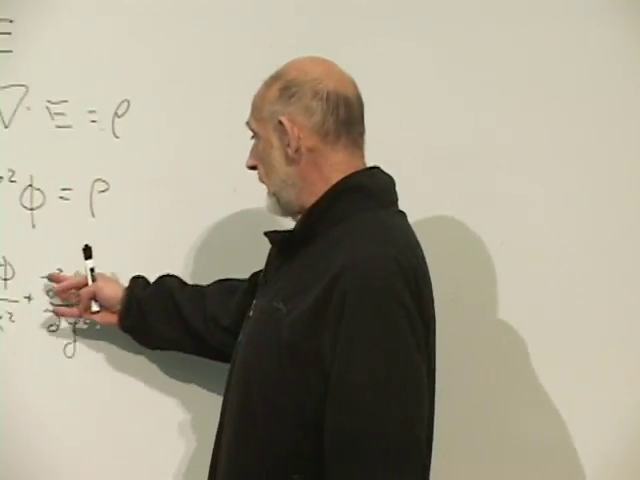
\includegraphics[width=0.70\textwidth]{lecture_08_figure_02.png}
  \caption{상대 부호가 마이너스인 것을 포함해 완성된 코시--리만 방정식 쌍.}
  \lectureframe{00:19:48}
  \label{fig:l08-cr-board}
\end{figure}

강의에서는 서로 연관된 용어를 간단히 구분한다. 유한 복소평면 전체에서 정칙인 함수는 전해석 함수다. 유리형 함수에는 고립된 극점이 있을 수 있다. 따라서 \(1/z\)는 \(z=0\)을 제외한 곳에서는 해석적이지만 전해석 함수는 아니다.

\section{조화 켤레와 등각 기하}

코시--리만 방정식은 결합된 1계 방정식이지만, 서로 분리된 2계 방정식을 함의한다. \(\partial_xu=\partial_yv\)를 \(x\)에 대해 미분하고, \(\partial_yu=-\partial_xv\)를 \(y\)에 대해 미분한 다음 더하면
\begin{align}
  \partial_x^2u&=\partial_x\partial_yv,\\
  \partial_y^2u&=-\partial_y\partial_xv,\\
  \therefore\qquad
  \partial_x^2u+\partial_y^2u&=0.
  \label{eq:l08-harmonic-u}
\end{align}
\(u\)와 \(v\)를 맞바꾸어 같은 논증을 반복하면
\begin{equation}
  \partial_x^2v+\partial_y^2v=0.
  \label{eq:l08-harmonic-v}
\end{equation}
따라서 해석 함수의 실수부와 허수부는 서로 조화 켤레다. 임의의 두 조화 함수가 자동으로 해석 함수를 이루는 것은 아니다. 두 함수는 여전히 \eqref{eq:l08-cauchy-riemann}로 연결되어야 한다.

\begin{figure}[H]
  \centering
  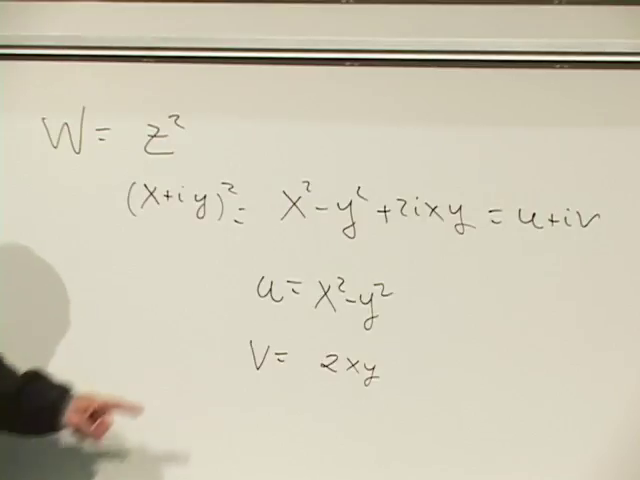
\includegraphics[width=0.68\textwidth]{lecture_08_figure_03.png}
  \caption{혼합 미분항이 상쇄되어 해석 사상의 한 성분에 대한 라플라스 방정식이 남는다.}
  \lectureframe{00:23:09}
  \label{fig:l08-harmonic-board}
\end{figure}

유용한 벡터 해석도 있다. \(\mathbf F=(u,-v)\)라면, 두 Cauchy--Riemann 방정식은 선택한 방향 규약에 따라 \(\mathbf F\)의 발산과 이차원 컬이 모두 사라짐을 나타낸다. 이것이 정전기학으로 돌아온다는 뜻이다.

\subsection{각도가 보존되는 이유}

두 개의 작은 복소 변위를 극형식으로 쓰자.
\begin{equation}
  \delta z=\rho e^{i\theta},
  \qquad
  \Delta z=\rho'e^{i\theta'}.
\end{equation}
두 변위의 비의 위상은 정확히 두 변위 사이의 각도인 \(\theta-\theta'\)이다. 해석 사상 아래에서는
\begin{equation}
  \frac{\delta w}{\delta z}
  =\frac{\Delta w}{\Delta z}
  =w'(z),
\end{equation}
미분 계수가 방향에 의존하지 않기 때문이다. 이를 정리하면
\begin{equation}
  \frac{\Delta z}{\delta z}
  =\frac{\Delta w}{\delta w}.
  \label{eq:l08-angle-ratio}
\end{equation}
양변의 위상이 같으므로 원래 선분 사이의 각도는 그 상 사이의 각도와 같다.

\begin{figure}[H]
  \centering
  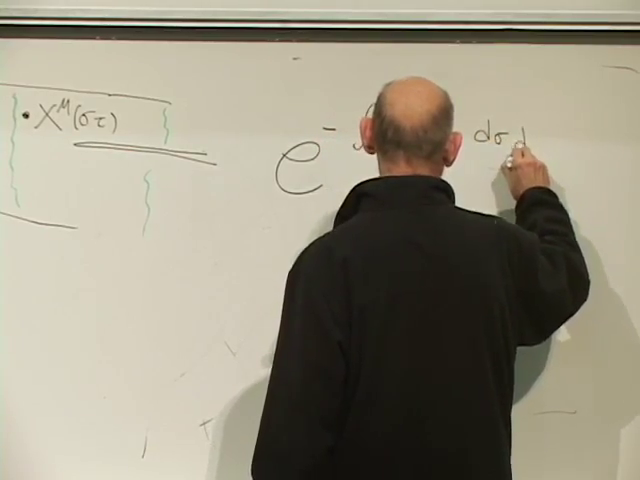
\includegraphics[width=0.70\textwidth]{lecture_08_figure_04.png}
  \medskip

  \begin{tikzpicture}[x=0.9cm,y=0.9cm,>=Latex]
    \begin{scope}
      \draw[->] (-0.2,0) -- (2.3,0);
      \draw[->] (0,-0.2) -- (0,2.1);
      \draw[very thick,blue!65!black,->] (0,0) -- (1.85,0.45)
        node[right] {\(\delta z\)};
      \draw[very thick,orange!75!black,->] (0,0) -- (0.72,1.65)
        node[above] {\(\Delta z\)};
      \draw (0.58,0.14) arc[start angle=14,end angle=66,radius=0.60];
      \node at (1.0,-0.55) {\(z\)-plane};
    \end{scope}
    \draw[->,thick] (3.0,0.9) -- (4.2,0.9)
      node[midway,above] {\(w(z)\)};
    \begin{scope}[xshift=5.0cm]
      \draw[->] (-0.2,0) -- (2.3,0);
      \draw[->] (0,-0.2) -- (0,2.1);
      \draw[very thick,blue!65!black,->] (0,0) -- (1.65,0.70)
        node[right] {\(\delta w\)};
      \draw[very thick,orange!75!black,->] (0,0) -- (0.48,1.62)
        node[above] {\(\Delta w\)};
      \draw (0.54,0.23) arc[start angle=23,end angle=74,radius=0.59];
      \node at (1.0,-0.55) {\(w\)-plane};
    \end{scope}
  \end{tikzpicture}
  \caption{칠판의 증명과 이를 국소적으로 깔끔하게 재구성한 그림. \(w'(z)\)를 곱하면 무한소 방향마다 같은 양만큼 회전하고 크기가 변하므로 방향 사이의 상대 각도가 보존된다.}
  \lectureframe{00:34:11}
  \label{fig:l08-angle-proof}
\end{figure}

이 국소 논증은 \(w'(z)\neq0\)을 가정한다. 임계점에서는 사상이 국소적으로 일대일이 아닐 수 있으므로 기하를 별도로 다루어야 한다. 그런 점을 제외하면 해석 사상과 방향을 보존하는 등각 사상은 국소적으로 같은 대상이다.

\section{눈에 익히기 위한 예제}

\subsection{제곱 사상과 복소켤레}

\(w=z^2\)일 때,
\begin{equation}
  (x+iy)^2=x^2-y^2+2ixy=u+iv,
\end{equation}
따라서
\begin{equation}
  u=x^2-y^2,
  \qquad
  v=2xy.
  \label{eq:l08-z-squared-components}
\end{equation}
\(u\)의 이계 도함수는 \(2\)와 \(-2\)이고, \(v\)의 이계 도함수들은 각각 사라진다. 두 함수 모두 조화 함수이며, 직접 미분해도 Cauchy--Riemann 방정식이 성립함을 확인할 수 있다.

\begin{figure}[H]
  \centering
  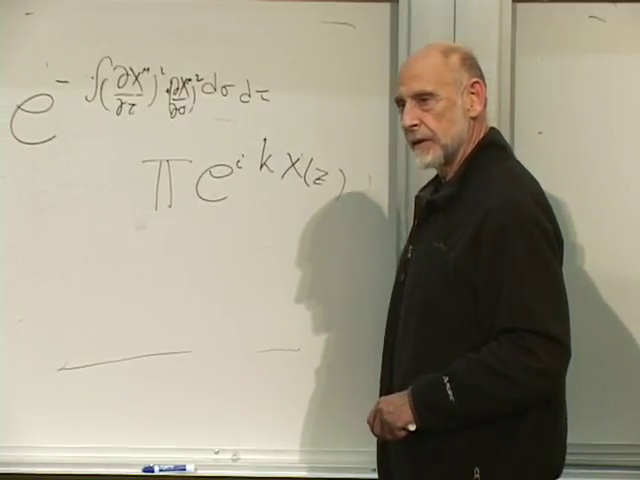
\includegraphics[width=0.72\textwidth]{lecture_08_figure_05.png}
  \caption{제곱 사상을 실수부와 허수부인 조화 성분으로 분해했다.}
  \lectureframe{00:36:45}
  \label{fig:l08-z-square-board}
\end{figure}

\begin{classroomqa}
\audiencequestion{\(1/z\)는 비해석 함수의 예인가요?
\lecturetimestamp{00:37:49}}
\lecturerresponse{한 점에서만 그렇다. \(z\neq0\)인 곳에서는 해석적이며 원점에 극점이 있다. 어디에서나 코시--리만 판정에 실패하는 사상을 보려면 복소켤레가 더 나은 예다.}
\end{classroomqa}

반면,
\begin{equation}
  w=\bar z=x-iy
  \qquad\Longrightarrow\qquad
  u=x,\quad v=-y
\end{equation}
이 사상은 방향을 뒤집는다. 그 도함수는 첫 번째 코시--리만 방정식에서 부호가 맞지 않으므로 \(z\)의 함수로서 해석적이지 않다.

\begin{figure}[H]
  \centering
  \includegraphics[width=0.62\textwidth]{lecture_08_figure_06.png}
  \caption{일부러 비해석적인 반례로 든 복소켤레.}
  \lectureframe{00:38:38}
  \label{fig:l08-conjugate-board}
\end{figure}

\subsection{지수 함수와 그 역함수}

\begin{classroomqa}
\audiencequestion{\(e^z\)가 해석 함수라면 그 역함수 \(\log z\)도 해석적이어야 하는 이유는 무엇인가요? \lecturetimestamp{00:40:38}}
\lecturerresponse{역함수가 존재하고 \(w'(z)\neq0\)인 곳에서는 그 도함수가 \(1/w'(z)\)이다. 따라서 방향 독립성이 보존된다. 로그 함수는 전역적으로 다가 함수이므로 가지를 하나 택하고 분기점과 분지선을 제외한다. 그 선택한 영역에서는 국소 등각 사상이 여전히 성립한다.}
\end{classroomqa}

오일러 공식으로부터
\begin{equation}
  w=e^z=e^{x+iy}
  =e^x(\cos y+i\sin y),
\end{equation}
따라서
\begin{equation}
  u=e^x\cos y,
  \qquad
  v=e^x\sin y.
  \label{eq:l08-exponential-components}
\end{equation}
예를 들어 \(\partial_xu=e^x\cos y=\partial_yv\)이고, 두 번째 코시--리만 방정식도 똑같이 직접 확인된다.

\begin{figure}[H]
  \centering
  \includegraphics[width=0.68\textwidth]{lecture_08_figure_07.png}
  \caption{지수 사상의 실수부와 허수부.}
  \lectureframe{00:42:23}
  \label{fig:l08-exponential-board}
\end{figure}

\section{반평면, 띠, 원통, 원판}

\subsection{로그 함수는 반지름을 시간으로 바꾼다}

다음과 같은 오른쪽 반평면을 취하고,
\(-\pi/2<\theta<\pi/2\)
다음과 같이 쓰자.
\begin{equation}
  z=re^{i\theta},
  \qquad
  w=\log z=\log r+i\theta.
  \label{eq:l08-log-map}
\end{equation}
이 반평면은 무한한 띠로 사상된다.
\begin{equation}
  -\frac{\pi}{2}<\operatorname{Im}w<\frac{\pi}{2}.
\end{equation}
\(\theta\)가 일정한 반직선은 수평선이 되고, \(r\)가 일정한 반원은 수직선이 된다. 원점은 \(\operatorname{Re}w=-\infty\)으로 사상되고, \(r=\infty\)는 \(\operatorname{Re}w=+\infty\)으로 사상된다.

\begin{figure}[H]
  \centering
  \includegraphics[width=0.75\textwidth]{lecture_08_figure_08.png}
  \caption{로그 함수는 오른쪽 반평면을 무한한 띠로 보낸다. 극좌표의 반직선과 반원은 직교하는 직사각형 격자가 된다.}
  \lectureframe{00:47:48}
  \label{fig:l08-log-strip-board}
\end{figure}

띠는 열린 끈의 표준 세계면이다. 띠의 유계 좌표는 끈을 따라가는 매개변수이고, 무한히 뻗은 방향으로의 평행 이동은 세계면 시간이다. 역 지수 사상 아래에서는 시간 평행 이동이 확대 \(z\mapsto e^a z\)로 바뀐다. 따라서 같은 대칭이 띠에서는 평행 이동으로, 반평면에서는 균일한 팽창으로 나타난다.

\begin{classroomqa}
\audiencequestion{\(r=1\) 같은 특정한 값은 어디로 가며, 띠의 좌표는 여전히 극좌표인가요? \lecturetimestamp{00:50:58}}
\lecturerresponse{반지름이 일정한 원은 \(\operatorname{Re}w=\log r\)에서 수직선이 된다. 특히 \(r=1\)는 중심선 \(\operatorname{Re}w=0\)로 사상된다. 극좌표는 \(z\)평면을 나타낸다. \(w\)평면에서는 보통의 직교 좌표를 사용한다. \((\log r,\theta)\)}
\end{classroomqa}

천공된 평면 전체에 \(\log z\)를 적용하면 각 좌표의 주기는 \(2\pi\)이다. 따라서 결과인 띠의 위쪽과 아래쪽 가장자리는 서로 동일시되어 무한 원통이 된다. 경계가 있는 반평면은 열린 끈의 세계면을 나타낸다. 경계가 없고 각도가 주기적인 전체 평면은 닫힌 끈의 원통을 나타낸다.

\begin{figure}[H]
  \centering
  \includegraphics[width=0.75\textwidth]{lecture_08_figure_09.png}
  \caption{반평면과 띠의 모습, 그리고 천공된 평면 전체를 닫힌 끈의 원통으로 만드는 주기적 동일시.}
  \lectureframe{00:54:23}
  \label{fig:l08-open-closed-board}
\end{figure}

\subsection{단위원판으로 보내는 케일리 사상}

선형 분수 사상, 즉 뫼비우스 사상은 오른쪽 반평면을 단위원판으로 보낸다.
\begin{equation}
  w=\frac{z-1}{z+1}.
  \label{eq:l08-cayley}
\end{equation}
이 사상은 \(z=0\)를 \(-1\)로, \(z=\infty\)를 \(+1\)으로 보내고, 허수축은 \(|w|=1\)로 보낸다. \(z=ir\)이면
\begin{equation}
  \left|\frac{ir-1}{ir+1}\right|=1.
\end{equation}
\(\operatorname{Re}z>0\)인 점들은 원판 안에 놓이며, 왼쪽 반평면은 원판 바깥으로 사상된다.
\editorialnote{강의 중 유도에서는 원판 내부로 사상된다고 설명하면서 역수 \((z+1)/(z-1)\)를 쓴다. 이 역수도 단위원 경계를 갖지만 오른쪽 반평면을 외부로 보낸다. 식 \eqref{eq:l08-cayley}은 설명한 기하와 일치하는 원판 내부 사상 규약이다.}

\begin{figure}[H]
  \centering
  \includegraphics[width=0.72\textwidth]{lecture_08_figure_10.png}
  \caption{단위원 경계를 만드는 선형 분수 사상. 칠판에 나타난 역수 규약은 원판 내부와 외부를 맞바꾼다.}
  \lectureframe{00:58:38}
  \label{fig:l08-cayley-board}
\end{figure}

뫼비우스 사상은 원과 직선으로 이루어진 일반화된 모임을 원과 직선으로 보낸다. 따라서 반평면의 반지름 방향 격자와 원형 격자는 원판 안의 서로 직교하는 두 호의 집합이 된다. 직선 지름은 중심이 무한대로 간 원의 극한에 해당한다.

\begin{classroomqa}
\audiencequestion{원판 안에 그린 곡선들은 정말 원인가요?
\lecturetimestamp{01:00:55}}
\lecturerresponse{그렇다. 원의 중심은 서로 다른 위치에 있으며, 그중에는 눈에 보이는 원판 바깥에 있는 것도 많다. 지름은 같은 원 집합에서 반지름이 무한대가 되는 극한이다.}
\end{classroomqa}

\begin{classroomqa}
\audiencequestion{원판 그림은 이것이 구면이라는 뜻인가요? 다른 반평면은 어디로 가나요? \lecturetimestamp{01:01:21}}
\lecturerresponse{여기 그림은 구면이 아니라 평평한 원판이다. 오른쪽 반평면은 원판 경계 안으로 사상되고 왼쪽 반평면은 바깥으로 사상된다. 복소평면 전체에 무한대점을 더하면, 확장된 평면을 입체 사영으로 구면에 나타낼 수 있다. 이는 전역적인 성질에 관한 별개의 진술이다.}
\end{classroomqa}

\begin{classroomqa}
\audiencequestion{원래의 방사형 선들과 반지름이 일정한 반원은 원판의 어떤 곡선에 대응하나요? \lecturetimestamp{01:02:59}}
\lecturerresponse{양의 실수축은 \(-1\)와 \(+1\)를 잇는 지름이 된다. 다른 반직선들도 같은 두 경계점을 잇는 원호가 된다. 반지름이 일정한 반원은 단위원에서 시작해 단위원에서 끝나는 직교 곡선 집합이 된다.}
\end{classroomqa}

\begin{figure}[H]
  \centering
  \includegraphics[width=0.72\textwidth]{lecture_08_figure_11.png}
  \caption{반평면의 직선과 반원은 원판 안에서 서로 직교하는 원과 직선의 집합으로 바뀐다.}
  \lectureframe{01:03:48}
  \label{fig:l08-circle-grid-board}
\end{figure}

\section{네 끈 세계면}

이제 산란으로 돌아가자. 열린 끈 두 개가 들어와 하나로 합쳐지고, 임의의 시간 동안 전파된 다음, 나가는 끈 두 개로 갈라진다. 띠 좌표에서 세계면은 양 끝에서 절개한 긴 띠처럼 보인다---이른바 ‘스포츠 밴드’ 그림이다. 중간 끈의 수명은 미리 정해져 있지 않다. 산란 진폭을 적분할 때 포함되는 여러 이력 중 하나다.

\((\sigma,\tau)\)를 세계면 좌표라고 하고,
\begin{equation}
  X^\mu=X^\mu(\sigma,\tau)
  \label{eq:l08-embedding}
\end{equation}
이 좌표가 시공간에서의 위치를 나타낸다고 하자. \(\sigma,\tau\)라는 표지는 2차원 매개변수 곡면에 속하고, 지표 \(\mu\)는 시공간 좌표를 나타낸다. 보손 이론에서는 \(\mu=0,\ldots,25\)이며, 초끈의 경우에는 시공간 좌표가 10개다.

위크 회전 뒤 자유 매장장의 유클리드 작용은 다음과 같다.
\begin{equation}
  S_E[X]
  =\frac{1}{4\pi\alpha'}\int_\Sigma d\sigma\,d\tau\,
  \left[
    \partial_\tau X^\mu\partial_\tau X_\mu
    +\partial_\sigma X^\mu\partial_\sigma X_\mu
  \right].
  \label{eq:l08-euclidean-action}
\end{equation}
이에 대응하는 경로 적분은 선택한 세계면을 시공간에 매장하는 모든 경우를 합한다.
\begin{equation}
  \int\mathcal D X\,e^{-S_E[X]}.
  \label{eq:l08-bare-worldsheet-integral}
\end{equation}

\begin{figure}[H]
  \centering
  \includegraphics[width=0.74\textwidth]{lecture_08_figure_12.png}
  \caption{완성된 양의 유클리드 세계면 가중치. 두 미분항은 모든 시공간 성분에 대해 합산한다.}
  \lectureframe{01:11:34}
  \label{fig:l08-action-board}
\end{figure}

절개된 띠에는 연결된 경계가 하나 있다. 따라서 등각 자유도를 이용해 이를 원판으로 나타낼 수 있다. 띠의 멀리 떨어진 네 끝은 경계 위의 네 표시점이 된다. 표시점의 위치를 변형하면 띠 좌표에서 합쳐짐과 분리 사이의 겉보기 간격은 달라지지만, 바탕이 되는 곡면이나 물리는 바뀌지 않는다.

\begin{figure}[H]
  \centering
  \includegraphics[width=0.76\textwidth]{lecture_08_figure_13.png}
  \caption{절개된 띠 세계면과 외부 끈의 경계점 네 개를 표시한 원판 표현.}
  \lectureframe{01:15:18}
  \label{fig:l08-bandage-disc-board}
\end{figure}

이 등각 사상을 그림으로 나타낼 때 쓰는 세부 격자선에는 물리적 의미가 없다. 중요한 것은 위상, 경계, 그리고 표시된 외부점이다. 같은 세계면을 서로 다른 채널의 모습으로 늘여 그릴 수 있지만, 새로운 상호작용이 생기는 것은 아니다.

\section{외부 상태를 경계 삽입으로 나타내기}

기본 적분 \eqref{eq:l08-bare-worldsheet-integral}만으로는 어떤 운동량이 들어오고 나가는지 알 수 없다. 운동량 \(k_i^\mu\)를 가진 스칼라 열린 끈 상태에 대해 경계에 다음 꼭짓점 연산자를 삽입하자.
\begin{equation}
  V_i(z_i)=e^{\,i k_i\cdot X(z_i)},
  \qquad
  k_i\cdot X=k_{i\mu}X^\mu.
  \label{eq:l08-vertex}
\end{equation}
점 \(z_i\)는 세계면 경계 위의 위치다. 시공간 좌표도, 운동량 방향도 아니다.

\begin{figure}[H]
  \centering
  \includegraphics[width=0.72\textwidth]{lecture_08_figure_14.png}
  \caption{부피 내부의 유클리드 가중치와 경계의 운동량 삽입 곱을 서로 구별되는 인자로 나타냈다.}
  \lectureframe{01:18:58}
  \label{fig:l08-vertex-board}
\end{figure}

\(n\)개의 외부 열린 끈에 대해 개략적인 처방은 다음과 같다.
\begin{equation}
  \begin{aligned}
    \mathcal A_n(k_1,\ldots,k_n)
    &=\int_{\mathcal M_{0,n}^{\partial}}\!d\mu(z_i)
      \int\mathcal D X\\
    &\quad\times e^{-S_E[X]}
      \prod_{i=1}^{n}e^{\,i k_i\cdot X(z_i)}.
  \end{aligned}
  \label{eq:l08-open-string-prescription}
\end{equation}
함수 적분은 매장 \(X^\mu\)에 대해 수행한다. 유한 차원 적분은 서로 동등하지 않은 경계 삽입 위치에 대해 수행한다. 강의에서와 같이 이 단계에서는 편극 인자와 게이지 고정 측도를 생략했다.
\editorialnote{완전한 게이지 고정 끈 진폭에는 적절한 고스트 기여, 상태에 따른 꼭짓점 인자, 결합 상수, 정규화도 들어간다. 식 \eqref{eq:l08-open-string-prescription}은 이 강의에서 다룬 매장장과 위치의 의존성을 나타낸다.}

\begin{classroomqa}
\audiencequestion{외부 운동량이 고정되어 있다면 왜 그 운동량에 대해 적분하나요? \lecturetimestamp{01:20:42}}
\lecturerresponse{운동량에 대해서는 적분하지 않는다. \(k_i\)는 산란 진폭의 고정된 표지다. 적분하는 것은 매장장과, 고정된 운동량이 삽입되는 세계면 위치 \(z_i\)다. 후자의 적분은 띠 그림에서 중간 끈의 수명에 대한 적분을 대신한다.}
\end{classroomqa}

\begin{classroomqa}
\audiencequestion{꼭짓점 인자의 곱은 경로 적분 안에 들어가나요? 작용의 일부인가요? \lecturetimestamp{01:21:39}}
\lecturerresponse{그 곱은 함수 적분 안에서 \(e^{-S_E}\)에 곱해진다. 인자들을 지수화해 작용에 국소화된 원천항을 더한 것으로 보아도 되지만, 개념적으로 이들은 자유 부피 작용의 일부가 아니라 꼭짓점 연산자다.}
\end{classroomqa}

\begin{figure}[H]
  \centering
  \includegraphics[width=0.76\textwidth]{lecture_08_figure_15.png}
  \caption{연속하는 외부 입자에 대한 인자 \(e^{ik_i\cdot X(z_i)}\)를 각각 따로 둔 경로 적분.}
  \lectureframe{01:23:23}
  \label{fig:l08-full-prescription-board}
\end{figure}

\begin{classroomqa}
\audiencequestion{세계면을 위크 회전한 뒤에도 \(e^{ik\cdot X}\)에 \(i\)가 남아 있는 이유는 무엇인가요? \lecturetimestamp{01:23:42}}
\lecturerresponse{회전은 세계면 시간을 바꾸며 부피 가중치를 \(e^{iS}\)에서 \(e^{-S_E}\)으로 바꾼다. 운동량 고유함수에 들어 있는 \(i\)는 시공간 운동량을 나타내는 푸리에 위상이다. 그 역할은 다르므로 그대로 남는다.}
\end{classroomqa}

\begin{classroomqa}
\audiencequestion{위치 \(z_i\)가 운동량 벡터의 방향을 정하나요? \lecturetimestamp{01:24:19}}
\lecturerresponse{아니다. 방향은 시공간 성분 \(k_i^\mu\)에 담긴다. 삽입점 \(z_i\)는 그 운동량이 세계면 기술에 어디에 들어가는지를 나타낸다. \(X^\mu(z_i)\)는 \(\mathcal D X\)에서 적분하는 장의 값들 중 하나다.}
\end{classroomqa}

\begin{classroomqa}
\audiencequestion{밴드 다리의 그림에서 보이는 각도가 물리적 운동량의 방향을 나타내나요? \lecturetimestamp{01:25:07}}
\lecturerresponse{아니다. 밴드는 매개변수 공간이지, 물리적 시공간에서 끈의 모습을 나타낸 그림이 아니다. 다리는 수평이나 기울어진 방향으로 그릴 수도 있고, 등각적으로 휘어 그릴 수도 있다. 물리적 방향은 성분 \(k^\mu\)으로 표현되고, \(X^\mu(\sigma,\tau)\)는 적분 변수다.}
\end{classroomqa}

\section{정전기학으로 보는 가우스 적분}

작용 \eqref{eq:l08-euclidean-action}은 모든 \(X^\mu\) 성분에 대해 이차식이고, 삽입항의 지수들을 작용과 결합하면 이 삽입항들은 선형 원천이 된다. 따라서 함수 적분은 가우스 적분이다. 안장점에서 각 시공간 성분은 다음과 같은 개략적인 푸아송 방정식을 만족한다.
\begin{equation}
  \nabla^2 X^\mu(z)
  \propto
  i\alpha'\sum_i k_i^\mu\,\delta(z-z_i),
  \label{eq:l08-electrostatic-source}
\end{equation}
원판 가장자리에서는 열린 끈 경계 조건을 적용한다. 각 \(X^\mu\)는 서로 독립인 정전기 퍼텐셜처럼 작용하고, 각 운동량 성분 \(k_i^\mu\)은 위치 \(z_i\)에 놓인 이에 대응하는 전하처럼 작용한다.

\begin{figure}[H]
  \centering
  \includegraphics[width=0.76\textwidth]{lecture_08_figure_16.png}
  \caption{경계 원천이 있는 원판을 시공간 성분마다 독립적인 2차원 정전기 문제 하나로 해석한다.}
  \lectureframe{01:28:58}
  \label{fig:l08-electrostatic-disc-board}
\end{figure}

정전기 문제를 풀고, 그 에너지를 계산하고, 음의 에너지를 지수화한 다음, 서로 동등하지 않은 전하 위치에 대해 적분한다. 표준 열린 끈 정규화에서 매장장 상관함수는 코바--닐센 인자를 준다.
\begin{equation}
  \left\langle\prod_i e^{\,ik_i\cdot X(z_i)}\right\rangle
  \propto
  (2\pi)^D\delta^{(D)}\!\left(\sum_i k_i\right)
  \prod_{i<j}|z_i-z_j|^{2\alpha' k_i\cdot k_j}.
  \label{eq:l08-koba-nielsen}
\end{equation}
델타 함수는 운동량 보존을 나타낸다. 곱에는 전하 사이의 정전기적 쌍 에너지가 들어 있다. 여기서 다루는 스칼라 경계 삽입 네 개의 경우, 위치 세 개를 고정하면 남은 적분은 앞선 강의에서 다룬 오일러 베타 적분이 된다.

\begin{classroomqa}
\audiencequestion{정전기 에너지는 26개인가요, 아니면 하나뿐인가요?
\lecturetimestamp{01:30:53}}
\lecturerresponse{시공간 성분마다 서로 독립적인 퍼텐셜과 장이 하나씩 있다. 정규 직교 표적공간 기저에서는 이들의 이차 에너지 사이에 교차항이 없으며, 지수화하기 전에 기여분들을 하나의 전체 작용에 더한다.}
\end{classroomqa}

\begin{classroomqa}
\audiencequestion{원판의 각 좌표는 물리적 산란각인가요? \lecturetimestamp{01:32:10}}
\lecturerresponse{아니다. 세계면 위치를 나타내는 매개변수다. 서로 동등하지 않은 위치의 조합은 중간 전파 구간과 관련되며 적분된다. 물리적 산란각은 고정된 운동량으로 만든 로런츠 불변량에 담긴다.}
\end{classroomqa}

\begin{classroomqa}
\audiencequestion{임계 차원에서 벗어나면 이 구성이 성립하지 않는 이유는 무엇인가요? \lecturetimestamp{01:32:35}}
\lecturerresponse{형식적인 가우스 적분만으로 일관성 조건을 모두 만족하는 것은 아니다. 게이지 고정은 등각 이상을 도입하며, 물질과 고스트의 기여는 임계 차원에서만 상쇄된다. 보손 끈에서는 \(D=26\)이고 초끈에서는 \(D=10\)이다. 이 상쇄가 없으면 양자 세계면의 등각 대칭이 사라진다.}
\end{classroomqa}

\begin{classroomqa}
\audiencequestion{이미 큰 공간 차원 세 개와 콤팩트한 여분 차원을 가정한 건가요? \lecturetimestamp{01:33:38}}
\lecturerresponse{아니다. 아직 콤팩트화는 이 구성에 들어오지 않았다. 이 단계에서 보손 좌표는 여전히 표적공간의 26개 방향 전체를, 초끈의 경우에는 10개 방향 전체를 누빈다. 그중 일부가 거시적으로 큰 상태로 남을 수 있는 방법은 다음 논의에서 다룬다.}
\end{classroomqa}

\begin{classroomqa}
\audiencequestion{정전기학과의 연관성은 좌표가 라플라스 방정식을 만족한다는 점뿐인가요? \lecturetimestamp{01:33:57}}
\lecturerresponse{그렇다. 삽입점에서 떨어진 곳에서는 각 \(X^\mu\)가 조화 함수이고, 꼭짓점 연산자는 델타 함수 원천을 제공한다. 정전기학 용어를 사용하든 말든, 이는 점전하가 있는 정적인 2차원 퍼텐셜의 경계값 문제와 수학적으로 동일하다.}
\end{classroomqa}

\subsection{등각 중복성과 모듈라이의 개수}

원판에는 3개의 실수 매개변수로 이루어진 등각 자기동형군 \(\mathrm{PSL}(2,\mathbb R)\)이 있다. 따라서 순서가 정해진 경계점 세 개를 편리한 위치에 고정할 수 있다. 외부 끈 네 개의 경우에는 네 번째 위치만 적분 대상으로 남는다. 순서가 정해진 경계 삽입이 \(n\)개라면 나무 수준에서 남는 실수 위치 적분은
\begin{equation}
  n-3
  \label{eq:l08-n-minus-three}
\end{equation}
개다.

\begin{classroomqa}
\audiencequestion{원판 둘레의 각 위치 네 개는 서로 독립인가요? \lecturetimestamp{01:34:37}}
\lecturerresponse{물리적으로는 그렇지 않다. 처음에는 위치 네 개를 쓰지만 원판의 등각 대칭으로 그중 아무 세 개나 원하는 위치에 둘 수 있다. 두 끈이 들어오고 두 끈이 나가는 진폭에서는 네 번째 위치의 상대적 위치만 남는다.}
\end{classroomqa}

\begin{figure}[H]
  \centering
  \includegraphics[width=0.72\textwidth]{lecture_08_figure_17.png}
  \caption{원판 경계의 삽입 네 개. 등각 자유도로 임의의 세 개를 고정하면 네 점 진폭의 모듈러스 하나가 남는다.}
  \lectureframe{01:35:18}
  \label{fig:l08-fix-three-board}
\end{figure}

\begin{classroomqa}
\audiencequestion{띠 그림에서 두 분리점이 같은 높이에 있지 않으면 어떻게 되나요? \lecturetimestamp{01:35:24}}
\lecturerresponse{등각 사상으로 겉보기의 높이 차이를 없앨 수 있다. 서로 다른 그림은 같은 모듈러스를 나타내는 좌표 표현이다. 불변인 적분은 남은 경계 위치, 또는 그와 동등하게 전파 구간에 대한 적분이다.}
\end{classroomqa}

\begin{classroomqa}
\audiencequestion{외부 입자가 더 많으면 위치 매개변수는 몇 개 남나요? \lecturetimestamp{01:36:00}}
\lecturerresponse{등각 대칭으로 삽입점 세 개를 고정하고 나머지 \(n-3\)개를 적분한다. 이것이 순서가 정해진 나무 수준 열린 끈 진폭에서 경계 모듈라이의 개수다.}
\end{classroomqa}

\begin{classroomqa}
\audiencequestion{이것은 M이론과 어떤 관계가 있나요?
\lecturetimestamp{01:36:37}}
\lecturerresponse{아직은 없다. 여기서 다룬 구성은 세계면 위의 섭동적 열린 끈 산란이다. M이론과의 관계에는 이후의 쌍대성과 비섭동적 개념이 필요하므로, 이 질문은 뒤로 미룬다.}
\end{classroomqa}

\begin{classroomqa}
\audiencequestion{수직 방향의 띠 그림이나 교차된 띠 그림은 서로 다른 계산을 뜻합니까? \lecturetimestamp{01:36:49}}
\lecturerresponse{아닙니다. 편리한 한 점을 고정하고 나머지 모듈러스가 전체 구간을 훑도록 둘 수 있습니다. 띠 그림과 원판 위 경계점 적분은 같은 적분을 서로 다르게 절단해 나타낸 것이며, 따라서 모든 외부 끈을 대칭적으로 다룰 수 있습니다.}
\end{classroomqa}

\section{처방으로 아직 해결되지 않는 문제}

원판 공식은 외부 끈이 더 많은 경우에도 즉시 확장됩니다. 꼭짓점 연산자를 더하고, 서로 동등하지 않은 경계 위치 \(n-3\)개에 대해 적분하면 됩니다. 이는 일관된 끈 모형을 위한 정밀한 나무 수준 처방이지만, 관측된 입자 물리학을 현실적으로 기술하는 모형은 아직 아닙니다. 단순한 보손 이론은 시공간 차원이 맞지 않고 다른 물리적 결함도 있습니다. 초끈 이론은 스펙트럼을 개선하고 임계 차원을 10으로 낮추지만, 여전히 6개의 공간 차원을 콤팩트화해야 합니다.

\begin{classroomqa}
\audiencequestion{이 단순한 모형은 입자 충돌 실험과 이미 일치합니까? \lecturetimestamp{01:39:06}}
\lecturerresponse{아닙니다. 공명 구조는 역사적으로 강입자 산란과 비슷했지만, 26차원 보손 모형은 관측된 입자를 직접 기술할 수 없습니다. 형식론은 이 모형의 산란 진폭을 정의합니다. 자연과 일치시키려면 현실적인 스펙트럼, 콤팩트화, 상호작용, 진공 선택이 필요합니다.}
\end{classroomqa}

\begin{classroomqa}
\audiencequestion{콤팩트화하면 여분의 차원이 줄어들고 현실적인 입자 데이터가 나옵니까? \lecturetimestamp{01:41:10}}
\lecturerresponse{거시적으로 유효한 차원을 줄이고 입자 스펙트럼과 게이지 군을 만들어 낼 수 있습니다. 수학적으로 어려운 문제의 상당 부분도 바로 여기서 시작됩니다. 일관된 콤팩트화는 많이 알려져 있지만, 관측된 기본 입자를 기술하는 유일한 모형을 선택하는 문제는 아직 해결되지 않았습니다.}
\end{classroomqa}

이 강의는 완성된 이론을 내세우기보다 이 차이를 강조합니다. 끈 이론의 구성은 수학적으로 명확하며 중력과 기하학에 관한 깊은 정보를 밝혀 왔지만, 그 구성의 다양성 자체가 물리학의 문제이기도 합니다.

\begin{classroomqa}
\audiencequestion{보손 끈 이론의 임계 차원이 26인 이유를 간단히 기억할 방법이 있습니까? \lecturetimestamp{01:43:19}}
\lecturerresponse{앞서 진동자 계산에서는 정규화된 영점 에너지 합 \(1+2+3+\cdots=-1/12\)을 사용했습니다. 횡방향 진동자의 기여에는 24개의 방향이 들어가며, 종방향 시공간 좌표 2개를 다시 포함하면 \(24+2=26\)가 됩니다. 이는 앞서 제시한 일관성 논증을 기억하기 위한 요령이지, 여기서 새로 유도하는 것은 아닙니다.}
\end{classroomqa}

\begin{classroomqa}
\audiencequestion{삽입된 운동량 벡터 \(k_i\) 자체도 양자화됩니까?
\lecturetimestamp{01:43:46}}
\lecturerresponse{비콤팩트 시공간에서는 운동량 벡터의 성분이 연속적입니다. 양자화되는 것은 진동자 준위이며, 따라서 허용되는 질량 제곱 스펙트럼이 양자화됩니다. 콤팩트 차원에서는 그에 대응하는 운동량 성분과 감김 성분이 양자화될 수 있지만, 그것은 다음 논의에서 다룹니다.}
\end{classroomqa}
